\documentclass[11pt,a4]{article} 
\usepackage[ansinew]{inputenc} %Schrifttyp und Umlaute
\usepackage{epsfig} %Nutzung von eps files
%\usepackage[dvips]{epsfig} %Nutzung von eps files
%\usepackage[final]{graphicx}    
%\usepackage[off]{auto-pst-pdf}     % necessary for psfrag to work
\usepackage{epstopdf} 
\usepackage{graphicx}

\usepackage[bf,sf,compact]{titlesec} 
\usepackage{fancyhdr} 
\usepackage{amsmath}
\usepackage{amssymb} %Symbole nach AMS
\usepackage{amstext}
\usepackage{theorem}
\usepackage{subfigure}
\usepackage{booktabs}

\usepackage{flafter}
\usepackage{exscale}
\usepackage{float}   % for minipages
\usepackage{psfrag}
\usepackage{listings}
\usepackage{color} %red, green, blue, yellow, cyan, magenta, black, white
\bibliographystyle{unsrt}

\setlength{\parindent}{0cm} 
\setlength{\textwidth}{16cm}
\setlength{\oddsidemargin}{0cm}  
\setlength{\voffset}{-2,8cm}  
\setlength{\textheight}{25cm} 
\setlength{\arrayrulewidth}{0,3mm} 
\setlength{\textheight}{25cm} 

\renewcommand{\labelenumi}{\alph{enumi})} 
\sloppy
\usepackage{xcolor}

% Linkcolour
\usepackage[	 
	colorlinks=true,
 	breaklinks=true,
	citecolor=black,
	linkcolor=black,	
	menucolor=black,	
	urlcolor=blue
]{hyperref}

\definecolor{mygreen}{RGB}{28,172,0} % color values Red, Green, Blue
\definecolor{mylilas}{RGB}{170,55,241}

\lstset{language=Matlab,%
    %basicstyle=\color{red},
    breaklines=true,%
    morekeywords={matlab2tikz},
    keywordstyle=\color{blue},%
    morekeywords=[2]{1}, keywordstyle=[2]{\color{black}},
    identifierstyle=\color{black},%
    stringstyle=\color{mylilas},
    commentstyle=\color{mygreen},%
    showstringspaces=false,%without this there will be a symbol in the places where there is a space
    numbers=left,%
    numberstyle={\tiny \color{black}},% size of the numbers
    numbersep=9pt, % this defines how far the numbers are from the text   
}


\begin{document} %hier geht es los

\thispagestyle{empty} 
\begin{tabular*}{16cm}{lr} \hline \\ %Tabelle mit zwei Spalten, in jeder Spalte eine minipage, neue Zeile mit \\
    \begin{minipage}{10cm} %Anfang minipage in linker Spalte, Breite 8cm
            \textsf{Technische Universit\"at Dortmund \\ %Schriftgröße smallface
            Department of Biochemical and Chemical Engineering \\
            Chair of Process Dynamics and Operations \\
            Prof.~Dr.~Sebastian Engell \\}
    \end{minipage} & %Ende minipage in linker Spalte
    \begin{minipage}{6cm} %Anfang minipage in rechter Spalte, Breite 8cm
            \setlength{\unitlength}{1cm} %Formatierung, Platzierung und Einfuegen des ASTLOGOS
            \begin{picture}(8,1) 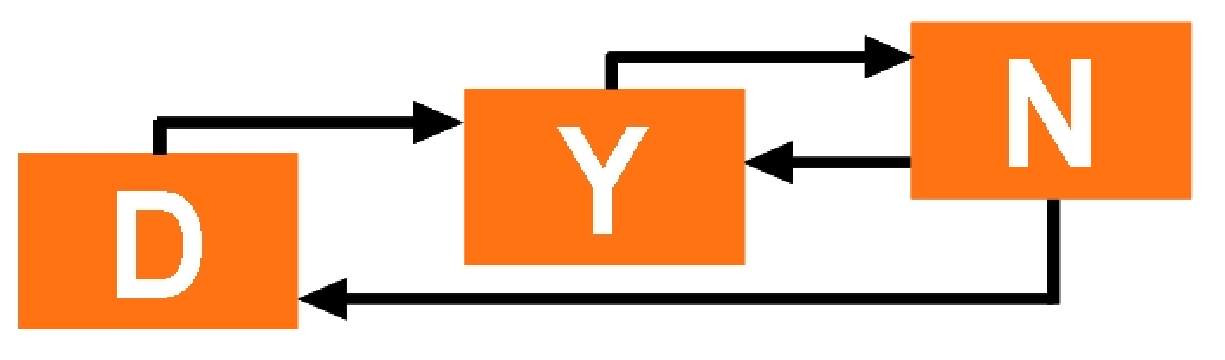
\epsfig{file= Astlogo.eps, width=5cm}
            \end{picture}\par
    \end{minipage} \\ \hline %Ende minipage in rechter Spalte
\end{tabular*} %Ende Tabelle




\vspace{5cm}

\begin{center} 

\LARGE{\bfseries DEVELOPMENT OF LOCAL POSITIONING SYSTEM FOR A PIPE-LESS PLANT\\

\vspace{0.25cm}
    Automation \& Robotics 
    
    Group Project SS18 \\}
    
\vspace{3cm}
\emph{Group Members:}\\[0.2cm]
Abdulrahman Abouelkhair(4511328)\\	                                         % Author info
Medhini Rajagopal Balamurugan(4511328)\\
Stefan Rottstegge(4511328)\\
Stephan Vette(4511328)\\[1.5cm]

\emph{Supervisors:}\\[0.2cm]
Afaq Ahmad \\ 
Marina Rantanen-Mod\'eer\\[1.5cm]	                                     % Supervisor info
\end{center}



%%%%%%%%%%%%%%%%%%%%%%%%%%%% ABSTRACT
\clearpage
\titleformat{\section}{\Large\bf}{\thesection:}{20pt}{}
\setcounter{enumi}{0} % !TeX encoding = UTF-8
\chapter*{\iftoggle{lang_eng}{Abstract}{Kurzfassung}}
Das ist die Kurzfassung. Hier sollte klar werden womit sich die Arbeit beschäftigt und die wichtigsten Aussagen sollen zusammengefasst werden. Richtwert is eine halbe Seite.

%%%%%%%%%%%%%%%%%%%%%%%%%%%%
\clearpage
\tableofcontents

\newpage
\listoffigures
\listoftables


\setlength{\textheight}{20cm}

\pagestyle{fancy} 
\lhead{Final report, TITLE, \today}
\chead{}
\rhead{Page \thepage}
\lfoot{}
\cfoot{}
\rfoot{} 
\renewcommand{\headrulewidth}{0.4pt} 

\setlength{\topmargin}{2cm} %oberer Rand bis Oberkante Kopfzeile

\makeatletter \def\usecounter#1{\@nmbrlisttrue\def\@listctr{#1}}
\makeatother 
\setcounter{figure}{0}
\setcounter{table}{0} 



%Introduction
\titleformat{\section}{\Large\bf}{\thesection}{20pt}{}
\section{Introduction} %

Add your name to the file name

%Theory
\clearpage
\titleformat{\section}{\Large\bf}{\thesection}{20pt}{}
\section{Pipeless Plant} %

\subsection{Existing setup}

\subsection{Problems with the Existing Setup}
..

zb
\begin{itemize}
\item Fish eye
\item Sunlight..
\end{itemize}

%%%%%%%%%%%%%%%%%%%%%%%%%%%%
\titleformat{\section}{\Large\bf}{\thesection}{20pt}{}
\section{Selection Process} 

About the 4 techniques..

\subsection[Triangulation]{Triangulation\footnote{Stefan}} %stefan
\subsubsection*{Summary}
Since our plant has a specified size in which the location of multiple objects has to be performed the method of Triangulation is one promising technic in which research was made. 
Triangulation was already a common principle of measurement in the 18th century and it´s divided between active and passive triangulation. Passive triangulation is a geometrical method based on two measurement stations which positions are known exactly. At these two measurement points angels of the desired point in space are measured to compute the localization in the specified coordinate system (x, y, z) with trigonometrical formulas.
With respect to the two measurement points which were already used in the 18th century nowadays two cameras are installed to perform a geographical method of 3D object-data estimation fig. \ref{Triangulation}.
\begin{figure}[!htbp]
\centering
\includegraphics[width = 16cm]{Pictures/Triangulation}
\caption{Passive Triangulation set-up with two cameras}
\label{Triangulation}
\end{figure}\\
To Solve the problem, it is necessary to know the parameters of the left and the right camera visualized in the figure. In theory the triangulation is trivial, since each and every point of the images of the respective cameras maps to a line in 3D space. If a pair of corresponding points, in the case of the pipes less plant it would be an AGV, is found the projection of a point x in 3D space can be computed. 
Active triangulation in comparison to passive triangulation needs one camera and at least one source of structured light (e.g. Laser). As the passive way here the geometrical location and orientation of the camera and light source is space need to be known. Two possible set-ups with either a laser point and a stripe as structured light are shown in fig. \ref{ative_Triangulation}.
\begin{figure}[!htbp]
\centering
\includegraphics[width = 16cm]{Pictures/acticetriangulation}
\caption{Active Triangulation}
\label{ative_Triangulation}
\end{figure}\\
To solve the active triangulation problem, the structured light has to point on object which location is desired to estimate, in the case of the pipe less plant it would be the AGV. If this point is found on the 2D image of the camera, a triangulation with basic trigonometrical formulas which are using the properties and parameters of the camera and light source can be performed and the position of the AGV is estimated. 
\subsubsection*{Implementation} 
One possible way to implement a solution for the passive triangulation is to attach 2 high resolution cameras with USB 3.0 for a fast data transmitting on two edges of the plant being not on each others opposite side as shown in fig. \ref{ ative_Triangulation_implementation}.
\begin{figure}[!htbp]
\centering
\includegraphics[width = 16cm]{Pictures/triangulationimplementatio}
\caption{Impmentation of passive triangulation}
\label{ative_Triangulation_implementation}
\end{figure}\\
The left and right camera are sequentially taking pictures which are transmitted to the plants computer where the image processing takes place. 

\subsubsection*{Pro and con}
\begin{table}[]
\centering
\begin{tabular}{|l|l|}
\hline
\multicolumn{2}{|c|}{\textbf{Passive Triangulation}}                                                                                                                  \\ \hline
\multicolumn{1}{|c|}{\textbf{Positive}}                                                                                    & \multicolumn{1}{c|}{\textbf{Negative}}   \\ \hline
Upgrade to USB 3.0 for faster data transmitting possible                                                                   & Light dependent                          \\ \hline
\begin{tabular}[c]{@{}l@{}}Upgrade to a camera with higher resolution to reduce \\ measurement error possible\end{tabular} & New concept of orientation may be needed \\ \hline
No Fish-Eye-Lense problem                                                                                                  & Limited range of observation             \\ \hline
Low cost                                                                                                                   &                                          \\ \hline
                                                                                                                           &                                          \\ \hline
\end{tabular}
\caption{Positive and Negative Points of Passive Triangulation}
\label{pro_con_passive_tri}
\end{table}
\begin{table}[]
\centering
\begin{tabular}{|l|l|}
\hline
\multicolumn{2}{|c|}{\textbf{Active Triangulation}}                                                                                                                     \\ \hline
\multicolumn{1}{|c|}{\textbf{Positive}}                                                                                    & \multicolumn{1}{c|}{\textbf{Negative}}     \\ \hline
Upgrade to USB 3.0 for faster data transmitting possible                                                                   & New unknown laser technology is needed     \\ \hline
\begin{tabular}[c]{@{}l@{}}Upgrade to a camera with higher resolution to reduce \\ measurement error possible\end{tabular} & High costs for several Laser (one per AGV) \\ \hline
Easy detection of laser points on camera image                                                                             & Laser needs to move while AGVs are moving  \\ \hline
                                                                                                                           & Limited range of observation               \\ \hline
                                                                                                                           & Light dependent                            \\ \hline
\end{tabular}
\caption{Positive and Negative Points of Active Triangulation}
\label{pro_con_active_tri}
\end{table}



\subsection{Pattern Recognition} %medhini
\subsubsection*{Summary} 
\subsubsection*{Implementation}
\subsubsection*{Pro and con}
..

\subsection[RFIS]{RFID\footnote{Stephan}} % stephan around 2 pages
\subsubsection*{Summary} 
One of the possible solutions to solve the challenging problem of indoor localization is the use of the Radio-frequency Identification (RFID) technology. The mainly areas of this technology is indeed still supply chains, transport, manufacturing, personnel access, animal tagging, toll collection \textcolor{red}{reference 4}, but has also become popular in localizing objects and persons. Where in the main applications only the identification has to be realized, also the strength of the signals is important to estimate the position of a certain object.\\
The main idea of those systems is that a reader detects a tag and reads its information. The technology can be divided into three main types: passive, semi-passive and active systems. A passive system, like it is been shown in fig. \ref{RFID_Passive}, consists of a reader, which is connected to an antenna and a computer and a passive tag.\\
\begin{figure}[!htbp]
\centering
\begin{minipage}{.5\textwidth}
\centering
\includegraphics[width = 7cm]{Pictures/RFID_Passive}%
\caption{Passive RFID System}
\label{RFID_Passive}
\end{minipage}%
\begin{minipage}{.5\textwidth}
\centering
\includegraphics[width = 7cm]{Pictures/RFID_Active}%
\caption{Active RFID System}
\label{RFID_Active}
\end{minipage}
\end{figure}\\
The system is called passive, because the power supply will be realized by the radio signal of the reader. In case where the tag is in the reading range of the reader, the tags gets enough power to send predefined information (for example ID) back. The active system (see fig.\ref{RFID_Active}) in comparison has an active tag which has an own power supply. The semi-passive tag has a battery build in that the the tag has more power to communicate, but is not used to generate radio frequency signals.\\ 
Another classification of RFID systems is the frequency of the radio waves. It can reach from 0.135 MHz (Low Frequency) to 5875 MHz (Super High Frequency). The table \ref{RFID_Systems} gives an overview about the systems related to reading ranges, reading rates and the ability to read near metal or water.\\
\begin{table}[!htbp]
\centering
\begin{tabular}{c}
\includegraphics[width = 9cm]{Pictures/RFID_Systems}
\end{tabular}
\caption{Overview RFID systems}
\label{RFID_Systems}
\end{table}\\
It can be seen that the passive systems in general have a smaller reading range then the active systems and has a bigger data rate. But it has also to be take into account, that passive tags a way cheaper then active tags.   
\subsubsection*{Implementation}
There are mainly two different ways to realize a localization system of the AGVs in the pipeless plant. Based on the fact that the plant has a size of 3 by 4 meter, the tracking can be carried out by passive system in which a couple of passive tags on the floor can be used as landmarks. In this case the reader plus the antenna would be placed on the AGV and localize with the help of the detected tags. The other systems consists of three or four reader in each corner of the plant and an active tag on each AGV. 

\subsubsection*{Pro and con}
Based on the made research, two tables with advantages and disadvantages of the two RFID systems are created.\\ 
\begin{table}[!htbp]
\centering
\begin{tabular}{|l|l|}
\hline
\multicolumn{2}{|c|}{\textbf{Active RFID system}}                                                                                                                                                                                \\ \hline
\multicolumn{1}{|c|}{\textbf{Pro}}                                                                                & \multicolumn{1}{c|}{\textbf{Con}}                                                                            \\ \hline
Light independent                                                                                                 & Prototype more expansive (3 reader + avtive tags)                                                            \\ \hline
Space unlimited                                                                                                   & \begin{tabular}[c]{@{}l@{}}Datarate is related to the amount of\\ detected tags a the same time\end{tabular} \\ \hline
\begin{tabular}[c]{@{}l@{}}Localization only has to be realized in\\ a bigger area - medium accuracy\end{tabular} & \begin{tabular}[c]{@{}l@{}}Anticollision need, cause more AGVs are\\ used at the same time\end{tabular}      \\ \hline
\begin{tabular}[c]{@{}l@{}}Wired communication between reader and \\ computer possible\end{tabular}               & \begin{tabular}[c]{@{}l@{}}Signal strength can be influenced by envirnonment\\ (metal or water)\end{tabular} \\ \hline
Simple algorithm (Trilateration)                                                                                  &                                                                                                              \\ \hline
\end{tabular}
\caption{Pro and cons of active RFID system}
\label{my-label}
\end{table}
\begin{table}[!htbp]
\centering
\begin{tabular}{|l|l|}
\hline
\multicolumn{2}{|c|}{\textbf{Passive RFID system}}                                                                                                                                                                                            \\ \hline
\multicolumn{1}{|c|}{\textbf{Pro}}                                                                                             & \multicolumn{1}{c|}{\textbf{Con}}                                                                            \\ \hline
Light independent                                                                                                               & \begin{tabular}[c]{@{}l@{}}Communication between AGV and computer \\ has to be realized\end{tabular}         \\ \hline
Space unlimited                                                                                                                & \begin{tabular}[c]{@{}l@{}}Data rate is related to the amount of\\ detected tags a the same time\end{tabular} \\ \hline
\begin{tabular}[c]{@{}l@{}}Localization only has to be realized between\\ four tags (small area) - high accuracy\end{tabular} & \begin{tabular}[c]{@{}l@{}}Anticollision need, cause more tags are\\ detected at the same time\end{tabular}  \\ \hline
Simple algorithm (Trilateration)                                                                                               &                                                                                                              \\ \hline
Prototype cheap (1 reader + passive tags)                                                                                      &                                                                                                              \\ \hline
\end{tabular}
\caption{Pro and cons passive RFID system}
\label{Pro and Cons of the passive RFID system}
\end{table}

\subsection{Map-Based Localization} %abdul
\subsubsection*{Summary} 
\subsubsection*{Implementation}
\subsubsection*{Pro and con}
..




%%%%%%%%%%%%%%%%%%%%%%%%%%%%
\titleformat{\section}{\Large\bf}{\thesection}{20pt}{}
\section{Theoretical Background} 

\subsection{Radio Frequency Identification}

\subsection{Trilateration}

\subsection{Simulation}

\subsection{...}

%%%%%%%%%%%%%%%%%%%%%%%%%%%%
\titleformat{\section}{\Large\bf}{\thesection}{20pt}{}
\section[Hardware]{Hardware\footnote{Stephan and Abdul}}

\subsection{RFID reader and antenna}

\subsection{RFID tag}

\subsection{Wifi modul}

%%%%%%%%%%%%%%%%%%%%%%%%%%%%
\titleformat{\section}{\Large\bf}{\thesection}{20pt}{}
\section[Simulation]{Simulation\footnote{Stephan}}

\subsection{Emulator}

\subsection{RSSI Measurements with real HW}

\subsection{Simulation with emulated data}

\subsection{Results}

%%%%%%%%%%%%%%%%%%%%%%%%%%%%
\titleformat{\section}{\Large\bf}{\thesection}{20pt}{}
\section{Implementation}

\subsection{Hardware (Abdul or Stephan)}

\subsection{Communication (Abdul and/or Stefan)}

\subsection{Initialization procedure (Stephan and Stefan)}

\subsubsection{Recording and filtering data (Stefan)}

\subsubsection{Analysing data (Stefan)}

\subsubsection{Estimation of position and orientation (Stephan)}

\subsection{Results}

\subsection{Improvements}



%%%%%%%%%%%%%%%%%%%%%%%%%%%%
\titleformat{\section}{\Large\bf}{\thesection}{20pt}{}
\section{Conclusion}\label{Sec_Conc}
% https://www.wikihow.com/Write-a-Conclusion-for-a-Research-Paper
% 1. Restate the topic. You should briefly restate the topic as well as explaining why it is important.
% 2. Restate your thesis. Aside from the topic, you should also restate or rephrase your thesis statement.
% 3. Briefly summarize your main points. Essentially, you need to remind your reader what you told them in the body of the paper.
% ( 4. Add the points up. If your paper proceeds in an inductive manner and you have not fully explained the significance of your points yet, you need to do so in your conclusion. )
% ( 5. Make a call to action when appropriate. If and when needed, you can state to your readers that there is a need for further research on your paper's topic. )
% 6. Answer the “so what” question.

% Phrases: ...A key limitation of the actual setup is that
The developed localization solution was for the pipeless plant, a prototype of a chemical production plant which has a size of 3 by 4 meter. In this plant the vessel will be transported by AGVs from one station to another. In the actual setup only a camera, which is installed above the plant, was used to detected the AGVs and estimate their positions. The problem with this technology is the bad detection of the LED pattern from the AGVs during bright light conditions and also the space limitation. Another big disadvantage is the big computation effort which makes the system also very slow. The main task of this project was to find an alternative tracking solution. During the project group phase differnt localization technologies were evaluated. With respect to the outcoming reseaches about triangulation, map-based-localizaion, pattern recognizion and localizaion via radio frequency identification the last RFID based localization of the AGV with passive tags as landmarks turned out to be the most promising among those four. With information of a similar project realized by the FH Dortmund a model to evaluate sample data and a localization algorithm was created in Matlab. This results of the simulation were promising and  therefore used during the decision making process about the actual hardware setup. With an demonstration board with the size of 30 cm x 30 cm the initialization procedure algorithm was implemented in which the AGV performes and 360$^\circ$ turn and estimates its position and its orientation based on measuremtns during this movement. With respect to this solutions it can be said that it is possible to assemble a reader on an AGV and detect passive tags with its antenna in a range of 14 cm. It also has been found out that an inconsistent realation between the revieved signal strength (RSSI) of the detected TAGs and the distance based on the RSSI is not generally trivial and was only solved in a rather simple and unriliable way during the project. Based on the results computed by the initializaion prcedure, it can be concluded that it is possible to estimate the position of the AGV with an average accuracy of aroung 2.5 cm and an estimation error of the orientation of around 23$^\circ$. Compared to the former localization set up this solutions, especially with respect to the orientation error, are not perfelty satisfying and just minimal requirements are fullfilled. The recieved data from the RFID reader have furthermore clearly shown that the anti-collision algorithm used by the reader leads to an unknown amount of time until each and every TAG in the detection area is identified. Summed up a model based demonstrator was realized which on the one hand does not improve the accuracy of the localizaion of the plant under good light conditions especially with respect to the orientation but on the other hand a promising technology for indoor localizaion with light independedcy, respectivelay cheap costs and highly scalability was found. 




%After the decision for a RFID system with passive tags as landmarks a prototype was build to verify the good solutions from the simulations. The implemented procedure was an initialization algorithm in which the the AGV makes an 360$^\circ$ turn and estimates its position and its orientation based on measurements during these turn. This project has shown that it is possible to put a reader on an AGV and detect passive tags with a reader and an antenna in an detection area of 14 cm. It has also been found out that there is inconsistent relation between the received signal strength (RSSI) of the detected tags and the distance between the tag and the reader. This leads to the fact that the estimation of the distance based on the RSSI is not trivial and was only solvable in a very simple and inaccurate way during the project. Based on the results from the initialization procedure, it can be concluded that it possible to estimate the position of the AGV with an average accuracy of around 2.5 cm and an estimation error of the orientation of around 23$^\circ$. This is not a very good results and fulfils only the minimal requirements. This project has also clearly shown that the anti-collision algorithm of the reader gives  very inefficient results and leads to an unknown amount of time until all tags in the detection area are identified. It was not possible to develop a running and faultless system, but is has been demonstrated that the system is light independent and space unlimited. Summing up all results, it can be concluded that the system is a promising technology for the indoor localizing on the small plant and gets rid of a lot of the current disadvantages. 

%%%%%%%%%%%%%%%%%%%%%%%%%%%%
\titleformat{\section}{\Large\bf}{\thesection}{20pt}{}

\section[Future Work]{Future Work\footnote{Stefan}} \label{Sec_fut}
After a proof-of-concept for an RFID based localizatin system has been build and a first demonstration set-up has been build the disadvantages and limitations of the prototype were evaluated. According to these results several points of improvement and extension were found and categorized into a hardware and a software section. 
\subsection{Hardware}
\begin{itemize}
\item The AGVs are feed by an included 12V battery which provides the power for all included electronical devices. This 12V power supply is available on board and is suggested to be used. Currently the WiFi-Module and the RFID-Reader are fed by an external powerbank since a 5V power supply is needed. In terms of one zentralized power supply a 12 V to 5 V converter can be installed and connected to the reader and wifi module.
\item As a first setup a demonstration area of 3 x 3 tags was build. In this rather small area the initializaion procedure was developed, but a real time localization while a path is followed by an AGV was not possible since the 30cm x 30cm was simply to small. For futrue research in terms of localizaion on a specified path additional TAGs can be included to the area of operation. Since the RFID concept is highly scalable the only change that needs to be made in the algorithm is the insertion of the additional TAG into the lookup table.
\item Currently the Robot No. 1 is the only AGV which is equipped with the RFID technology. To run the plant with multible AGVs the remaining robots needs to be upgraded.\\
\end{itemize}
\subsection{Software}
\begin{itemize}
\item During the initalizatin procedure a 360$^\circ$ turn is performed. The desired turn around 45$^\circ$ is realized by a driving time of 1125 ms. But it needs to be said that this movement is highly dependend on disturbances like changing battery charge and plant underground. For the future developers it is suggested to use the encoders of the robot wheels as a determination of the orientation instead of the parameter time.
\item As an alternative localization technology was found several code lines in the current code can be deleted since the camera and image processing is simply not used anymore. With a clean code an improvement of processing time will be achieved.
\item As a last point it can be said that even though a localization with RFID is now possible the results are not 100 percent realiable and the accuracy especially with respect to the orientation is not satisfying so far. As an improvement the triangulation algorithm has to be optimized and or a second RFID-antenna has to be added under the AGV to reduce measurment errors.
\end{itemize}

%%%%%%%%%%%%%%%%%%%%%%%%%%%%
\titleformat{\section}{\Large\bf}{\thesection}{20pt}{}
\include{sections/References}

%%%%%%%%%%%%%%%%%%%%%%%%%%%%
\titleformat{\section}{\Large\bf}{\thesection}{20pt}{}
\section{Appendixes}

\subsection{Appendix A: Emulator RFID data (Matlab)}\label{Sec_AppA}
\scriptsize
\lstinputlisting{code/Emulator.m}



\label{LetzteSeite} %marker letzte Seite


\end{document}

\label{LetzteSeite} %marker letzte Seite

%%%%%%%%%%%%%%%%%%%%%     EXTRA HELP    %%%%%%%%%%%%%%%%%%%%%%%%%%%%%%%%%%%%%%%%
% TO ADD A PICTURE..

% \begin{figure}[h!]
%   \includegraphics[width=\linewidth]{boat.jp g}
%   \caption{A boat.}
%   \label{fig:boat1}
% \end{figure}


% TO ADD A TABLE..

% \begin{table}[h!]
% \centering
%  \begin{tabular}{||c c c c||} 
%  \hline
%  Col1 & Col2 & Col2 & Col3 \\ [0.5ex] 
%  \hline\hline
%  1 & 6 & 87837 & 787 \\ 
%  2 & 7 & 78 & 5415 \\
%  3 & 545 & 778 & 7507 \\
%  4 & 545 & 18744 & 7560 \\
%  5 & 88 & 788 & 6344 \\ [1ex] 
%  \hline
%  \end{tabular}
%  \caption {Should be a caption}
% \end{table}

